% Generic template
%
% Author: In this template, the places where you need to add information
%         (or delete line) are indicated by {???}.  Mostly the information
%         required is obvious, but some explanations are given in lines starting
% Author:
% All other lines should be ignored.  After editing, there should be
% no instances of ??? after this line.

% use option [preprint] to remove info line at bottom:

\documentclass[dvips]{imsart}
\usepackage[pdftex]{graphicx}
\DeclareGraphicsExtensions{.jpg,.pdf,.png,.gif,.ps,.pdf,.eps}
\usepackage{listings}
\usepackage[pdftex,colorlinks=true,linkcolor=blue,citecolor=blue,urlcolor=blue]{hyperref}

%\usepackage{amsthm,amsmath,natbib}
%\RequirePackage[colorlinks,citecolor=blue,urlcolor=blue]{hyperref}

% use this package if hyperref and natbib is used:
%\RequirePackage{hypernat}

% provide arXiv number if available:
%\arxiv{math.PR/0000000}

% put your definitions there:
\startlocaldefs
\endlocaldefs

\usepackage{eso-pic}
\newcommand\BackgroundPic{
\put(0,0){
\parbox[b][\paperheight]{\paperwidth}{%
\vfill
\centering

\includegraphics[width=\paperwidth,height=\paperheight,
keepaspectratio]{img/draft.png}%
\vfill
}}}

\begin{document}
% add Draft
%\AddToShipoutPicture{\BackgroundPic}
\begin{frontmatter}

% "Title of the Paper"
\title{IBM Rational Rhapsody build optimization}
%\thankstext{t1}{}
\runtitle{IBM Rational Rhapsody build optimization}
%\vspace{1cm}
%
\includegraphics[width=6cm,angle=0]{img/Logo_company.jpg}
% indicate corresponding author with \corref{}
% \author{\fnms{John} \snm{Smith}\thanksref{t2}\corref{}\ead[label=e1]{smith@foo.com}\ead[label=e2,url]{www.foo.com}}
% \thankstext{t2}{Thanks to somebody}
% \address{line 1\\ line 2\\ \printead{e1}\\ \printead{e2}}

\author{\fnms{Eric}
\snm{Keller}\ead[label=e1]{ekeller@hamilton-medical.ch}}
\and
\author{\fnms{Lars}
\snm{Schmohl}\ead[label=e2]{lschmohl@hamilton-medical.ch}\ead[label=e3,url]{http://www.hamilton-medical.com/}}
\address{\printead{e1} \printead{e2}}
%\address{\printead{e1}}
\address{\printead{e3}}
\runauthor{Eric Keller, Lars Schmohl}

\begin{abstract}
Nowadays, software engineers have to deal with increasingly complex problems,
so that they do not want to spend their time on setting up a proper build
process. Knowing that existing tools were created in order to increase the
developer productivity, these mechanisms, unfortunately are not natively integrated in Rational Rhapsody.
Intra components, classes and Rhapsody files dependencies among all the Rhapsody models, permit efficient incremental builds.
Parallel or distribute compilation of build processes, reduce the overall
building time. Using the GNU make tool, combined with a GNU gcc based compiler, 
Rational Rhapsody for C++ build processes can easily be tuned up. 
This approach should also be applicable to other programming languages and
different build processes. As a result, we reduced our compilation time by a
factor two. Developers are able to work on multiple Rhapsody models
without taking care of the dependencies, when performing an incremental build.
``Build and run your program often'', said Bruce Douglass. Adjusting our tools
to obtain an optimized work flow is part of this success.
\end{abstract}

%\begin{keyword}[class=AMS]
%\kwd[Primary ]{}
%\kwd{}
%\kwd[; secondary ]{}
%\end{keyword}

%\begin{keyword}
%\kwd{}
%\kwd{}
%\end{keyword}

% history:
% \received{\smonth{1} \syear{0000}}
\tableofcontents
\end{frontmatter}

%/---------------------\
% Introduction, presentation
%\---------------------/
\section{Introduction}
\subsection{Hamilton-Medical AG}

\emph{Hamilton-Medical}, an independent joint stock company with a strong
operational link to Hamilton in Bonaduz, is specialized in ventilator systems and their
accessories. The company's products are used in intensive care units, recovery
rooms and nursing homes.

\emph{Hamilton-Medical} mission is to provide care with safe and reliable
respiratory therapy devices through development, manufacturing, and distribution of innovative products and
services, for ventilated patients in hospitals and sub acute care facilities, worldwide.

The Hamilton Group, is a privately owned company that now employs approximately
1,000 people. Bonaduz is the major pole of production employing more than 400 people.
\emph{Hamilton-Medical} is a member of Hamilton Group, employing 60 people.

\subsection{Platform C Software}

The platform C project is actively developed by 7 software engineers.
The target architecture is PPC32 running under \emph{WindRiver VxWorks}
Operating System.

The former \emph{Ilogix/Telelogic}, now \emph{IBM Rational Rhapsody} tool was
integrated to our development environment 4 years ago. The platform C project
is composed of 29 Rhapsody models (.rpy), organized in 51 libraries and 35
executables components, generating approximately 1 million line of C++ code.

Generating and building this code without any optimization took more than one
hour.

%/---------------------\
% Problems - Limitation
%\---------------------/
\section{Development with IBM Rational Rhapsody}
% several models composing libraries and executable
% Rhapsody model organization => a directory per model component
% a Makefile per component model
% no direct link to other component makefile, no dependency is managed through
% makefile
\subsection{Rhapsody models structure}
As explained in the IBM Rational Rhapsody Team Collaboration Guide
\cite{RhpTeamColla-09}, we adopted the multiple Rational Rhapsody project
structure, meaning several libraries are used by executables. Each and every
entity became a Rhapsody Model, stored as an .rpy project.

Each component generates its source code in a separate directory getting the
component name. All the component directories are gathered into a common
``generate'' directory.

Rhapsody generates a Makefile per component, which is located at the same level
as the generated source code.

\label{ProjStruct}
\begin{figure}[ht]
\centering
  \framebox{
    \begin{minipage}{12cm}
     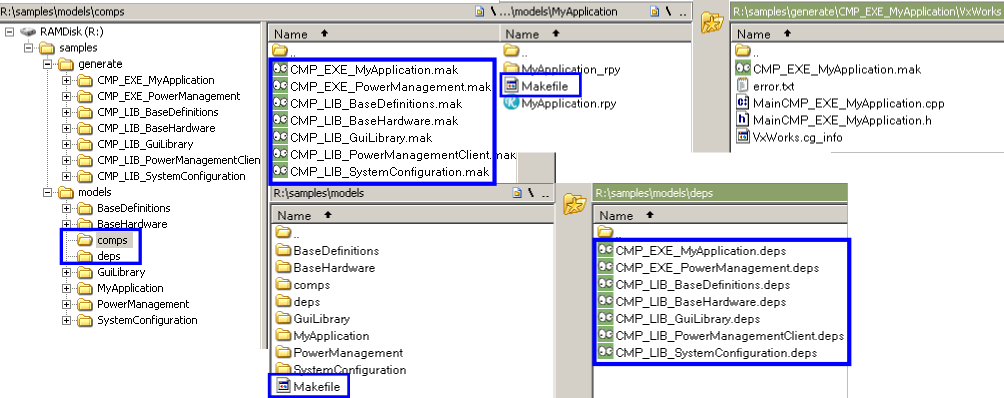
\includegraphics[width=\textwidth]{img/structure.png}
    \end{minipage}}
 \caption{Rhapsody projects structure}
 \label{fig:projStruct}
\end{figure}

Relative path definitions are used in order to stay flexible, no matter where
the project is checked out.
\begin{itemize}
    \item Property PathInProjectList Enum "Absolute, Relative" "Relative"
    \item Property ReferenceUnitPath Enum "Absolute, Relative" "Relative"
    \item Property ComponentIsSavedUnit    Bool    "True"
\end{itemize}

\subsection{Out of the box limitation}
During development phases, one of the most used Rhapsody operations, is the
code generation followed by the code compilation. Depending on size and
structure of one project, this tasks can take a considerable amount of time.

In this section we will present the problems and limitations we encountered
while using the Rhapsody tool. Some problems are directly related to Rhapsody
for instance, the time opening / generating a larger model. Other limitations
are not foreseen originally by Rhapsody, but can easily be configured, like
inter-class dependencies.

\subsubsection{Code generation}
% generation time to open a model for generation
% no possibility to select one class/package to generate with rhpCL
% class being in the scope of 2 different component is not automatically
% generated for both component (only the active c omponent!)
There are two methods to start code generation with Rhapsody:
\begin{itemize}
  \item using the GUI \emph{Code - Generate - Configuration} (Ctrl+F7)
  \item using the command line tool \emph{RhapsodyCL.exe}
  \begin{verbatim}
RhapsodyCL.exe -lang=cpp -cmd=open myModel.rpy -cmd=generate
myComponent myConfiguration
\end{verbatim}
\end{itemize}

On the one hand, generating the source code from the Rhapsody GUI is
definitively faster, when your model is currently open in a Rhapsody GUI
instance. On the other hand, generating the source code from the RhapsodyCL
takes a considerable amonunt of time since the whole model is loaded first,
using the \emph{-hiddenui} option, and then the code is generated.

The new feature coming with Rhapsody 7.4, ``generate with dependencies'',
unfortunately only works with a Gui instance of Rhapsody.

As described in the Rational Rhapsody command-line interface (CLI)
\cite{RhpUsrGuide-09} generating the source code without starting the Gui
instance is useful for nightly build procedure, or continuous build integration.
 
\subsubsection{Build with dependencies}
% with the version 7.4 7.5 the build with dependency feature still limited,
Building with dependencies is the key of incremental builds which spares much
time while compiling, and insure that the obtained executable integrate all the
modifications.

Processing ``full builds'' (cleaning the object files, and re-compiling), instead of properly
setting the appropriate dependencies to use ``incremental builds'', is
definitively a waste of time.

There are several level of dependencies when scoping Rhapsody Projects:
\begin{description}
  \item[between components] and other components, for example when an executable
  uses libraries. The dependency can be local, meaning both of the components
  are part of the same Rhapsody model. Yet usually the components are depending
  on other components populated from another Rhapsody Model.
  \item[between classes], basically when including a header file, a C++ class
  depends on the modification of the class it includes, on both the header (.h)
  and the source file (.cpp).
  \item[between generated source code and rhapsody files], modification on the
  Rhapsody model, has to be reflected on the generated source files.
\end{description}

Rhapsody uses two different mechanisms to handle these dependencies. The first,
internal procedure, which are part of the Rhapsody tool and require a Gui
instance to be started\footnote{using the Java API can also trigger some
functionalities}. The second, makefiles are generated in order to build
executable, these makefiles can be used without any instance of the
Rhapsody tool.

In recent version, the developer is able to generate / build
components with dependencies. This procedure is unfortunately only integrated
to Rhapsody Gui version. No additional makefile containing
component dependencies is generated so far.

In order to build components, Rhapsody uses an alternative mechanism, a
Makefile, which contains some basic dependencies between classes, but this
approach stays limited to classes being in the same component scope.

Finally, the dependency between the Rhapsody model files and the generated
source code, is some internal process again, which update a set of classes to
be generated according to their timestamps.

\subsubsection{Multiple CPU load}
% multiple CPU during generation, compilation is unused 
Nowadays hosts computer have at least dual core CPU. When using the
available computing resources, the code generation and compilation procedure
time is divided by the number of available processors. Per default, Rhapsody
does not take into account the number of processors while generating or
compiling C++ code.

Using Rhapsody to manage large projects compilation time becomes an
issue. A distribute compilation integration, reduces this time.
%/---------------------\
% Optimisations
%\---------------------/
\section{Workarounds and optimizations}
In the following sections, we give concrete solutions, to the problem we
encountered while managing the Platform C project with Rational Rhapsody.
These workarounds and optimizations are working for our project, with few
adaptation, any C/C++ Rhapsody driven project is able to profit from them.

Concerning the other programing languages supported by Rhapsody, Java and Ada,
finding the appropriate tools (Ant\footnote{Apache Ant is a Java-based build
tool. In theory, it is kind of like Make}, Ivy\footnote{Ivy is a very powerful
dependency manager oriented toward Java dependency management}, \ldots) and
adapting the concept should be possible.

\subsection{Additional Makefile generation}
% using intern structure of the model to parse the dependent components
% autogen.pl script
Relying on additional GNU makefiles solved two of the dependencies problems.
These makefiles can be used in a terminal (without any Rhapsody instance), or
from a Rhapsody Gui Instance. Additionally it could directly be integrated to
our nightly builds and continuous integration processes.

We did not used the Rhapsody Java API neither the VBA scripting, since both
are requiring to load the Rhapsody Model, before starting any operation. To
save time we use a Perl script operating on the Rhapsody file directly.

\subsubsection{Platform C: parent Makefiles}
% project component diagram
The main idea is to generate a ``parent makefile'', located in the project
directory gathering all the Rhapsody models, in our case the \emph{models}
directory. This makefile contains unique targets for every component of each
model composing the project. The components targets have as prerequisite their
dependencies to the other components.

As a parent makefile, it also contains a target with the complete list of
components which compose the final software product.

For achieving this goal, the autogen.pl Perl script, opens all the available
*.rpy files to extract the existing components and their dependencies in the
*.cmp files.

\paragraph{Extracting the Rhapsody components} 
In order to generate the parent makefile we extracted the existing
components from every Rhapsody model (*.rpy): 

\lstset{frame=shadowbox, numbers=left, breaklines=true,
caption=HardwareDefinitions.rpy}
\begin{lstlisting}
[...]
- Components = { IRPYRawContainer
    - size = 2;
    - value =
    { IComponent
    - fileName = "CMP_LIB_HardwareDefinitions";
    - _id = GUID 8f4607d2-9a63-4f0a-a453-9249b4fd3f96;
    }
    { IComponent
    - fileName = "CMP_LIB_BaseDefinitions";
    - _persistAs = "../../BaseDefinitions/BaseDefinitions_rpy";
    - _id = GUID 572539ee-e597-47a6-a8a3-1e23da4fefd9;
    - _isReference = 1;
    }
}
[...]
\end{lstlisting}

The components matching our interest, are the ones belonging to the current
Rhapsody model. Every component saved ``persistent'' (- \_persistAs) in another
location, are irrelevant since these are belonging to another Rhapsody model.

\paragraph{Extracting the components dependencies}
The next operation consist of opening consecutively all the associated
components we listed (stored in files with the .cmp extension) to determine
the dependency to components defined  in another Rhapsody model.

Depending on the Rhapsody model structure, there are two methods defining
a component dependency:
\begin{itemize}
  \item extract the dependencies from the component diagram
  \item extract the dependencies from the include paths defined in the
  component configuration
\end{itemize}

\lstset{frame=shadowbox, numbers=left, breaklines=true,
caption=snippet of CMP\_LIB\_HardwareDefinitions.cmp dependencies from component
diagram}
\begin{lstlisting}
[...]
{ IDependency
    - _id = GUID 28f91050-b6a6-11de-8252-001a92daad3c;
    - _myState = 2048;
    - _name = "CMP_LIB_BaseDefinitions";
    - Stereotypes = { IRPYRawContainer
[...]
}
\end{lstlisting}
\lstset{frame=shadowbox, numbers=left, breaklines=true,
caption=snippet of CMP\_LIB\_HardwareDefinitions.cmp dependencies form include
paths}
\begin{lstlisting}
[...]
- _includePath = "../../generate/CMP_LIB_BaseDefinitions/";
[...]
\end{lstlisting}

\paragraph{Components dependencies}
% defines the inter component dependency
By processing the obtained information, we are able to create a dependency
file (located in a models/deps directory) and a component makefile (located in a
models/comps directory) per Rhapsody model. The dependency file lists every
component and its dependencies to other components:

\lstset{frame=shadowbox, numbers=left, breaklines=true,
caption=snippet of models/deps/BaseHardware.deps Fig:~\ref{fig:projStruct} on
~\pageref{fig:projStruct}}
\begin{lstlisting}
[...]
CMP_LIB_BaseHardware.a=\
 CMP_LIB_BaseDefinitions.a\
 CMP_LIB_SystemConfiguration.a

CMP_EXE_BaseHardwareTest.vxe=\
 CMP_LIB_BaseHardware.a
[...]
\end{lstlisting}

The makefile contains a target per component having all the component
dependencies as prerequisites. The corresponding dependency file is required by the component makefile.
\label{compMake}
\lstset{frame=shadowbox, numbers=left, breaklines=true,
caption=snippet of models/comps/BaseHardware.mak Fig:~\ref{fig:projStruct} on
~\pageref{fig:projStruct}}
\begin{lstlisting}
[...]
# dependencies
include ./deps/BaseHardware.deps

BaseHardware: CMP_LIB_BaseHardware.a \
    CMP_EXE_BaseHardwareTest.vxe

# the $(CMP_EXE_BaseHardwareTest.vxe) is defined in the
# included ./deps/CMP_EXE_BaseHardware.deps
CMP_EXE_BaseHardwareTest.vxe: $(CMP_EXE_BaseHardwareTest.vxe)
    cd BaseHardware && make CMP_EXE_BaseHardwareTest.vxe
   
CMP_LIB_BaseHardware.a: $(CMP_LIB_BaseHardware.a)
    cd BaseHardware && make CMP_LIB_BaseHardware.a
[...]
\end{lstlisting}

\paragraph{Rhapsody Models affiliation}
% contains all the component from all concerned Rhapsody models
In addition to the list of executable components composing the software
project, the parent makefile includes every component makefiles:

\lstset{frame=shadowbox, numbers=left, breaklines=true,
caption=snippet of models/Makefile Fig:~\ref{fig:projStruct} on
~\pageref{fig:projStruct}}
\begin{lstlisting}
[...]
project: \
    CMP_EXE_PowerManagment.vxe \
    CMP_EXE_MyApplication.vxe
   
include ./comps/BaseDefinitions.mak
include ./comps/BaseHardware.mak
include ./comps/PowerManagment.mak
include ./comps/SystemConfiguration.mak
include ./comps/GuiLibrary.mak
include ./comps/MyApplication.mak
[...]
\end{lstlisting}

\subsubsection{Platform C: models Makefiles}
% component list, sorted components
% without dependency
% calls the Rhapsody generated makefile => // distrubute compilation
Finally the analysis of the Rhapsody model permits to generate a model
makefile located in the same directory than the Rhapsody model itself.
This Makefile contains the same targets as the component makefile
\ref{compMake}, but implements the call to the Rhapsody generated makefile located in the
/generate/Component/Configuration directory.

In this model makefile, we added the dependency rule between the
Rhapsody files and the generated source code. The \emph{RHPDEPS}
definition, contains all the *.sbs and *.cmp file. When the developer saves a
Rhapsody model, the timestamps are modified and the code will automatically be
regenerated.

\label{parallelCompil}
\lstset{frame=shadowbox, numbers=left, breaklines=true,
caption=snippet of models/BaseHardware/Makefile Fig:~\ref{fig:projStruct} on
~\pageref{fig:projStruct}, label=modelMakefile}
\begin{lstlisting}
MODEL    := BaseHardware
ARCH    := VxWorks
# enable the --jobs option if the host PC
# has more than 1 CPU
ifeq ($(shell if [ "${NUMBER_OF_PROCESSORS}" -gt "1" ];then; echo "YES";fi),YES)
    PARALLEL="-j $(NUMBER_OF_PROCESSORS)"
endif

RHPDEPS:=$(wildcard ./$(MODEL)_rpy/PKG_Design/*.sbs) $(wildcard
./$(MODEL)_rpy/*.cmp)

rhp.g: $(RHPDEPS)
    @echo "generate the source code, one of the Rhapsody file was modified:$(RHPDEPS)"
    @make generate
    touch $@
    @echo "auto-generation done"

all: common
common: CMP_LIB_BaseHardware.a
tests: CMP_UEXE_BaseHardwareTest.vxe
[...]

CMP_LIB_BaseHardware.a: rhp.g
    make -f ../../generate/CMP_LIB_BaseHardware/$(ARCH)/CMP_LIB_BaseHardware.mak CPU=PPC32 TOOL=gnu $(PARALLEL) all

CMP_UEXE_BaseHardwareTest.vxe: rhp.g
   	make -f ../../generate/CMP_UEXE_BaseHardwareTest/$(ARCH)/CMP_UEXE_BaseHardwareTest.mak CPU=PPC32 TOOL=gnu $(PARALLEL) all
[...]
\end{lstlisting}

\subsection{Rhapsody Makefile improvements}
% class has its dependency on other class level even if a class is not in the
% scope or in the same model
Concerning dependencies between classes, we decided to improve the Rhapsody
makefile, by updating it directly in the site.prp file.
We use the GNU gcc \cite{GNUgcc-08} pre-compiler feature \emph{``-MM -MT''}
providing the complete list of dependencies of a class.

\lstset{frame=shadowbox, numbers=left, breaklines=true,
caption=snippet of site.prp: ``Property MakeFileContent MultiLine''
replacing:\$OMContextMacros}
\begin{lstlisting}
[...]
#######################################
#### Context generated dependencies ###
# Add .d to Make's recognized suffixes.
SUFFIXES += .d
#We don't need to clean up when we're making these targets
NODEPS:=cleanall clean distclean
#These are the dependency files, which make will clean up after it creates them
DEPFILES:=$(patsubst %.o,%.d,$(OBJS))

#Don't create dependencies when we're cleaning
ifeq (0,$(words $(findstring $(MAKECMDGOALS),$(NODEPS))))
-include $(DEPFILES)
endif

#This is the rule for creating the dependency files
./%.d: ./%.cpp
    @echo \"making dependencies for $<\"
    @$(CXX) $(C++HAMFLAGS) $(ConfigurationCPPCompileSwitches) -MM -MT
    '$(patsubst %.cpp,%.o,$<)' $< > $@

#This rule does the compilation
./%.o: ./%.cpp ./%.d ./%.h
    @$(CREATE_OBJ_DIR)
    @echo \"Compiling $<\"
	@$(CXX) $(C++HAMFLAGS) $(ConfigurationCPPCompileSwitches) -o $@ -c $<
[...]
\end{lstlisting}

An additional file, with the .d extension, is generated before compilation
time. It contains all the dependency a class can have, regardless of the
component scope. As a result, this dependencies file is set as a prerequisite to
the object files so that an object has to be recompiled, if one of its dependencies have
changed.

\lstset{frame=shadowbox, numbers=left, breaklines=true,
caption=snippet of CGPIODevice.d}
\begin{lstlisting}
CGPIODevice.o: CGPIODevice.cpp CGPIODevice.h \
[...]
  PSS_BaseHardware.h DevTraceConfigBaseHardware.h \
  ../../CMP_LIB_BaseDefinitions/VxWorks/CSignalSemaphore.h \
  ../../CMP_LIB_BaseDefinitions/VxWorks/CBase.h \
  ../../CMP_LIB_BaseDefinitions/VxWorks/CStringOperations.h \
  ../../CMP_LIB_SystemConfiguration/VxWorks/CSystemConfiguration.h
\end{lstlisting}

\subsection{Parallel / distribute compilation}
\subsubsection{The GNU make: --jobs option}
GNU make knows how to execute several commands at once.
Normally, make will execute only one command at a time, waiting for it to finish before executing the next.
However, the `-j' or `--jobs' option tells make to execute many commands
simultaneously\cite{GNUmake-06}.

Using this GNU make feature reduced the generation time of all our models by
half. On the one hand, we were able to generate simulatenously two Rhapsody
models one on each CPU\footnote{We are still using Dual cores, but the division factor
would be 4 using quadcores}. On the other hand, parallelisation of each
compilation divides the overall build time by two for the same reasons.

\begin{description}
\item[under Windows] the environement variable: \emph{NUMBER\_OF\_PROCESSORS} is
set to the number of available CPUs
\item[under Unix] the following command returns you the number of processors:
\begin{verbatim}
cat /proc/cpuinfo | grep "^processor" | wc -l
\end{verbatim}
\end{description}

We are using this information to enable parallel code generation and
compilation, see the \$(PARALLEL) definition in the
models/BaseHardware/Makefile \ref{parallelCompil}.

\subsubsection{Samba DistCC}
distcc is a program to distribute builds of C, C++ code across several machines on a network.
distcc should always generate the same results as a local build, is simple to
install, use and is usually much faster than a local
compile\cite{sambaDistcc-09}.

One of the last build optimisation, is to use the distcc tool, enabled to
distribute our builds over a compilation farm. This last operation reduced
the overall compilation time, especially when distributing the pre-processor
operation using the pump mode.

Still the effectiveness of distcc relies on the number of processor composing
the compilation farm and the frequency of the CPU.

\section{Conclusions}
As a Conclusion, the presented improvements we made for our Platform C project
did reduce the overall time by 50\%, introducing proper
dependencies structures permitted incremental builds, sparing some additional
time, without doubting that part of the software was built with out-dated code.

Using IBM Rational Rhapsody as a development tool with the goal to achieve
shorter time to market our products was the appropriate move. Invest a small
amount of time to configure it, so you can profit from an efficient
build process in the future.

\bibliographystyle{plain}
\bibliography{ekeller-ibm-inno}

\end{document}
 